\chapter{Debugging, condition handling, and defensive
programming}\label{debugging}

What happens when something goes wrong with your R code? What do you do?
What tools do you have to address the problem? This chapter will teach
you how to fix unanticipated problems (debugging), show you how
functions can communicate problems and how you can take action based on
those communications (condition handling), and teach you how to avoid
common problems before they occur (defensive programming).

Debugging is the art and science of fixing unexpected problems in your
code. In this section you'll learn the tools and techniques that help
you get to the root cause of an error. You'll learn general strategies
for debugging, useful R functions like \texttt{traceback()} and
\texttt{browser()}, and interactive tools in RStudio.

Not all problems are unexpected. When writing a function, you can often
anticipate potential problems (like a non-existent file or the wrong
type of input). Communicating these problems to the user is the job of
\textbf{conditions}: errors, warnings, and messages.

\begin{itemize}
\item
  Fatal errors are raised by \texttt{stop()} and force all execution to
  terminate. Errors are used when there is no way for a function to
  continue. \index{errors} \indexc{stop()}
\item
  Warnings are generated by \texttt{warning()} and are used to display
  potential problems, such as when some elements of a vectorised input
  are invalid, like \texttt{log(-1:2)}.
\item
  Messages are generated by \texttt{message()} and are used to give
  informative output in a way that can easily be suppressed by the user
  (\texttt{?suppressMessages()}). I often use messages to let the user
  know what value the function has chosen for an important missing
  argument.
\end{itemize}

Conditions are usually displayed prominently, in a bold font or coloured
red depending on your R interface. You can tell them apart because
errors always start with ``Error'' and warnings with ``Warning
message''. Function authors can also communicate with their users with
\texttt{print()} or \texttt{cat()}, but I think that's a bad idea
because it's hard to capture and selectively ignore this sort of output.
Printed output is not a condition, so you can't use any of the useful
condition handling tools you'll learn about below.

Condition handling tools, like \texttt{withCallingHandlers()},
\texttt{tryCatch()}, and \texttt{try()} allow you to take specific
actions when a condition occurs. For example, if you're fitting many
models, you might want to continue fitting the others even if one fails
to converge. R offers an exceptionally powerful condition handling
system based on ideas from Common Lisp, but it's currently not very well
documented or often used. This chapter will introduce you to the most
important basics, but if you want to learn more, I recommend the
following two sources:

\begin{itemize}
\item
  \href{http://homepage.stat.uiowa.edu/~luke/R/exceptions/simpcond.html}{\emph{A
  prototype of a condition system for R}} by Robert Gentleman and Luke
  Tierney. This describes an early version of R's condition system.
  While the implementation has changed somewhat since this document was
  written, it provides a good overview of how the pieces fit together,
  and some motivation for its design.
\item
  \href{http://www.gigamonkeys.com/book/beyond-exception-handling-conditions-and-restarts.html}{\emph{Beyond
  Exception Handling: Conditions and Restarts}} by Peter Seibel. This
  describes exception handling in Lisp, which happens to be very similar
  to R's approach. It provides useful motivation and more sophisticated
  examples. I have provided an R translation of the chapter at
  \url{http://adv-r.had.co.nz/beyond-exception-handling.html}.
\end{itemize}

The chapter concludes with a discussion of ``defensive'' programming:
ways to avoid common errors before they occur. In the short run you'll
spend more time writing code, but in the long run you'll save time
because error messages will be more informative and will let you narrow
in on the root cause more quickly. The basic principle of defensive
programming is to ``fail fast'', to raise an error as soon as something
goes wrong. In R, this takes three particular forms: checking that
inputs are correct, avoiding non-standard evaluation, and avoiding
functions that can return different types of output.

\paragraph{Quiz}

Want to skip this chapter? Go for it, if you can answer the questions
below. Find the answers at the end of the chapter in
\hyperref[debugging-answers]{answers}.

\begin{enumerate}
\def\labelenumi{\arabic{enumi}.}
\item
  How can you find out where an error occured?
\item
  What does \texttt{browser()} do? List the five useful single-key
  commands that you can use inside of a \texttt{browser()} environment.
\item
  What function do you use to ignore errors in block of code?
\item
  Why might you want to create an error with a custom S3 class?
\end{enumerate}

\paragraph{Outline}

\begin{enumerate}
\def\labelenumi{\arabic{enumi}.}
\item
  \hyperref[debugging-techniques]{Debugging techniques} outlines a
  general approach for finding and resolving bugs.
\item
  \hyperref[debugging-tools]{Debugging tools} introduces you to the R
  functions and Rstudio features that help you locate exactly where an
  error occurred.
\item
  \hyperref[condition-handling]{Condition handling} shows you how you
  can catch conditions (errors, warnings, and messages) in your own
  code. This allows you to create code that's both more robust and more
  informative in the presence of errors.
\item
  \hyperref[defensive-programming]{Defensive programming} introduces you
  to some important techniques for defensive programming, techniques
  that help prevent bugs from occurring in the first place.
\end{enumerate}

\hyperdef{}{debugging-techniques}{\section{Debugging
techniques}\label{debugging-techniques}}

\begin{quote}
``Finding your bug is a process of confirming the many things that you
believe are true --- until you find one which is not true.''

---Norm Matloff
\end{quote}

Debugging code is challenging. Many bugs are subtle and hard to find.
Indeed, if a bug was obvious, you probably would've been able to avoid
it in the first place. While it's true that with a good technique, you
can productively debug a problem with just \texttt{print()}, there are
times when additional help would be welcome. In this section, we'll
discuss some useful tools, which R and RStudio provide, and outline a
general procedure for debugging. \index{debugging} \index{bugs}

While the procedure below is by no means foolproof, it will hopefully
help you to organise your thoughts when debugging. There are four steps:

\begin{enumerate}
\def\labelenumi{\arabic{enumi}.}
\item
  \textbf{Realise that you have a bug}

  If you're reading this chapter, you've probably already completed this
  step. It is a surprisingly important one: you can't fix a bug until
  you know it exists. This is one reason why automated test suites are
  important when producing high-quality code. Unfortunately, automated
  testing is outside the scope of this book, but you can read more about
  it at \url{http://r-pkgs.had.co.nz/tests.html}.
\item
  \textbf{Make it repeatable}

  Once you've determined you have a bug, you need to be able to
  reproduce it on command. Without this, it becomes extremely difficult
  to isolate its cause and to confirm that you've successfully fixed it.

  Generally, you will start with a big block of code that you know
  causes the error and then slowly whittle it down to get to the
  smallest possible snippet that still causes the error. Binary search
  is particularly useful for this. To do a binary search, you repeatedly
  remove half of the code until you find the bug. This is fast because,
  with each step, you reduce the amount of code to look through by half.

  If it takes a long time to generate the bug, it's also worthwhile to
  figure out how to generate it faster. The quicker you can do this, the
  quicker you can figure out the cause.

  As you work on creating a minimal example, you'll also discover
  similar inputs that don't trigger the bug. Make note of them: they
  will be helpful when diagnosing the cause of the bug.

  If you're using automated testing, this is also a good time to create
  an automated test case. If your existing test coverage is low, take
  the opportunity to add some nearby tests to ensure that existing good
  behaviour is preserved. This reduces the chances of creating a new
  bug.
\item
  \textbf{Figure out where it is}

  If you're lucky, one of the tools in the following section will help
  you to quickly identify the line of code that's causing the bug.
  Usually, however, you'll have to think a bit more about the problem.
  It's a great idea to adopt the scientific method. Generate hypotheses,
  design experiments to test them, and record your results. This may
  seem like a lot of work, but a systematic approach will end up saving
  you time. I often waste a lot of time relying on my intuition to solve
  a bug (``oh, it must be an off-by-one error, so I'll just subtract 1
  here''), when I would have been better off taking a systematic
  approach.
\item
  \textbf{Fix it and test it}

  Once you've found the bug, you need to figure out how to fix it and to
  check that the fix actually worked. Again, it's very useful to have
  automated tests in place. Not only does this help to ensure that
  you've actually fixed the bug, it also helps to ensure you haven't
  introduced any new bugs in the process. In the absence of automated
  tests, make sure to carefully record the correct output, and check
  against the inputs that previously failed.
\end{enumerate}

\hyperdef{}{debugging-tools}{\section{Debugging
tools}\label{debugging-tools}}

To implement a strategy of debugging, you'll need tools. In this
section, you'll learn about the tools provided by R and the RStudio IDE.
RStudio's integrated debugging support makes life easier by exposing
existing R tools in a user friendly way. I'll show you both the R and
RStudio ways so that you can work with whatever environment you use. You
may also want to refer to the official
\href{http://www.rstudio.com/ide/docs/debugging/overview}{RStudio
debugging documentation} which always reflects the tools in the latest
version of RStudio.

There are three key debugging tools:

\begin{itemize}
\item
  RStudio's error inspector and \texttt{traceback()} which list the
  sequence of calls that lead to the error.
\item
  RStudio's ``Rerun with Debug'' tool and
  \texttt{options(error = browser)} which open an interactive session
  where the error occurred.
\item
  RStudio's breakpoints and \texttt{browser()} which open an interactive
  session at an arbitrary location in the code.
\end{itemize}

I'll explain each tool in more detail below.

You shouldn't need to use these tools when writing new functions. If you
find yourself using them frequently with new code, you may want to
reconsider your approach. Instead of trying to write one big function
all at once, work interactively on small pieces. If you start small, you
can quickly identify why something doesn't work. But if you start large,
you may end up struggling to identify the source of the problem.

\subsection{Determining the sequence of calls}

The first tool is the \textbf{call stack}, the sequence of calls that
lead up to an error. Here's a simple example: you can see that
\texttt{f()} calls \texttt{g()} calls \texttt{h()} calls \texttt{i()}
which adds together a number and a string creating a error:
\index{call stack} \indexc{traceback()}

\begin{Shaded}
\begin{Highlighting}[]
\NormalTok{f <-}\StringTok{ }\NormalTok{function(a) }\KeywordTok{g}\NormalTok{(a)}
\NormalTok{g <-}\StringTok{ }\NormalTok{function(b) }\KeywordTok{h}\NormalTok{(b)}
\NormalTok{h <-}\StringTok{ }\NormalTok{function(c) }\KeywordTok{i}\NormalTok{(c)}
\NormalTok{i <-}\StringTok{ }\NormalTok{function(d) }\StringTok{"a"} \NormalTok{+}\StringTok{ }\NormalTok{d}
\KeywordTok{f}\NormalTok{(}\DecValTok{10}\NormalTok{)}
\end{Highlighting}
\end{Shaded}

When we run this code in Rstudio we see:

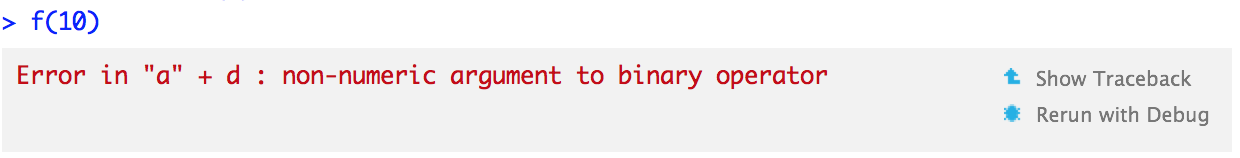
\includegraphics[width=4.35in]{screenshots/traceback-hidden.png}

Two options appear to the right of the error message: ``Show Traceback''
and ``Rerun with Debug''. If you click ``Show traceback'' you see:

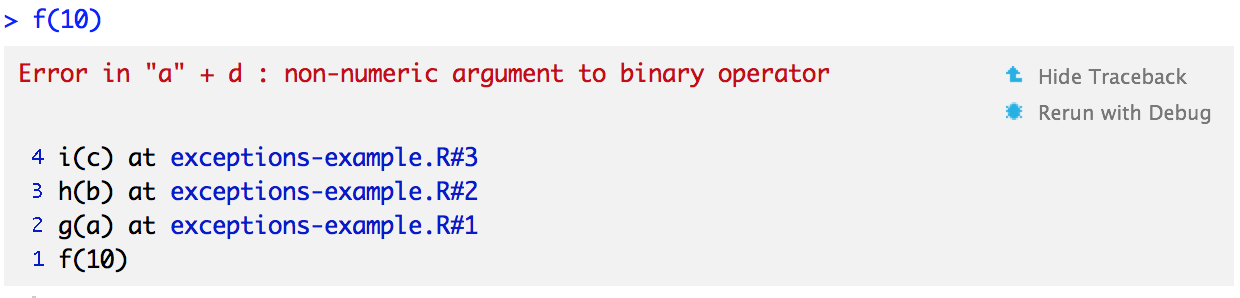
\includegraphics[width=4.35in]{screenshots/traceback-shown.png}

If you're not using Rstudio, you can use \texttt{traceback()} to get the
same information:

\begin{Shaded}
\begin{Highlighting}[]
\KeywordTok{traceback}\NormalTok{()}
\CommentTok{# 4: i(c) at exceptions-example.R#3}
\CommentTok{# 3: h(b) at exceptions-example.R#2}
\CommentTok{# 2: g(a) at exceptions-example.R#1}
\CommentTok{# 1: f(10)}
\end{Highlighting}
\end{Shaded}

Read the call stack from bottom to top: the initial call is
\texttt{f()}, which calls \texttt{g()}, then \texttt{h()}, then
\texttt{i()}, which triggers the error. If you're calling code that you
\texttt{source()}d into R, the traceback will also display the location
of the function, in the form \texttt{filename.r\#linenumber}. These are
clickable in Rstudio, and will take you to the corresponding line of
code in the editor.

Sometimes this is enough information to let you track down the error and
fix it. However, it's usually not. \texttt{traceback()} shows you where
the error occurred, but not why. The next useful tool is the interactive
debugger, which allows you to pause execution of a function and
interactively explore its state.

\subsection{Browsing on error}

The easiest way to enter the interactive debugger is through RStudio's
``Rerun with Debug'' tool. This reruns the command that created the
error, pausing execution where the error occurred. You're now in an
interactive state inside the function, and you can interact with any
object defined there. You'll see the corresponding code in the editor
(with the statement that will be run next highlighted), objects in the
current environment in the ``Environment'' pane, the call stack in a
``Traceback'' pane, and you can run arbitrary R code in the console.
\index{debugger, interactive}

As well as any regular R function, there are a few special commands you
can use in debug mode. You can access them either with the Rstudio
toolbar (\includegraphics[width=2.48in]{screenshots/debug-toolbar.png})
or with the keyboard:

\begin{itemize}
\item
  Next, \texttt{n}: executes the next step in the function. Be careful
  if you have a variable named \texttt{n}; to print it you'll need to do
  \texttt{print(n)}.
\item
  Step into, \includegraphics[width=0.24in]{screenshots/step-into.png}
  or \texttt{s}: works like next, but if the next step is a function, it
  will step into that function so you can work through each line.
\item
  Finish, \includegraphics[width=0.24in]{screenshots/finish-loop.png} or
  \texttt{f}: finishes execution of the current loop or function.
\item
  Continue, \texttt{c}: leaves interactive debugging and continues
  regular execution of the function. This is useful if you've fixed the
  bad state and want to check that the function proceeds correctly.
\item
  Stop, \texttt{Q}: stops debugging, terminates the function, and
  returns to the global workspace. Use this once you've figured out
  where the problem is, and you're ready to fix it and reload the code.
\end{itemize}

There are two other slightly less useful commands that aren't available
in the toolbar:

\begin{itemize}
\item
  Enter: repeats the previous command. I find this too easy to activate
  accidentally, so I turn it off using
  \texttt{options(browserNLdisabled = TRUE)}.
\item
  \texttt{where}: prints stack trace of active calls (the interactive
  equivalent of \texttt{traceback}).
\end{itemize}

To enter this style of debugging outside of RStudio, you can use the
\texttt{error} option which specifies a function to run when an error
occurs. The function most similar to Rstudio's debug is
\texttt{browser()}: this will start an interactive console in the
environment where the error occurred. Use
\texttt{options(error = browser)} to turn it on, re-run the previous
command, then use \texttt{options(error = NULL)} to return to the
default error behaviour. You could automate this with the
\texttt{browseOnce()} function as defined below: \indexc{options(error)}

\begin{Shaded}
\begin{Highlighting}[]
\NormalTok{browseOnce <-}\StringTok{ }\NormalTok{function() \{}
  \NormalTok{old <-}\StringTok{ }\KeywordTok{getOption}\NormalTok{(}\StringTok{"error"}\NormalTok{)}
  \NormalTok{function() \{}
    \KeywordTok{options}\NormalTok{(}\DataTypeTok{error =} \NormalTok{old)}
    \KeywordTok{browser}\NormalTok{()}
  \NormalTok{\}}
\NormalTok{\}}
\KeywordTok{options}\NormalTok{(}\DataTypeTok{error =} \KeywordTok{browseOnce}\NormalTok{())}

\NormalTok{f <-}\StringTok{ }\NormalTok{function() }\KeywordTok{stop}\NormalTok{(}\StringTok{"!"}\NormalTok{)}
\CommentTok{# Enters browser}
\KeywordTok{f}\NormalTok{()}
\CommentTok{# Runs normally}
\KeywordTok{f}\NormalTok{()}
\end{Highlighting}
\end{Shaded}

(You'll learn more about functions that return functions in
\hyperref[functional-programming]{Functional programming}.)

There are two other useful functions that you can use with the
\texttt{error} option:

\begin{itemize}
\item
  \texttt{recover} is a step up from \texttt{browser}, as it allows you
  to enter the environment of any of the calls in the call stack. This
  is useful because often the root cause of the error is a number of
  calls back. \indexc{recover()}
\item
  \texttt{dump.frames} is an equivalent to \texttt{recover} for
  non-interactive code. It creates a \texttt{last.dump.rda} file in the
  current working directory. Then, in a later interactive R session, you
  load that file, and use \texttt{debugger()} to enter an interactive
  debugger with the same interface as \texttt{recover()}. This allows
  interactive debugging of batch code. \indexc{dump.frames()}

\begin{Shaded}
\begin{Highlighting}[]
\CommentTok{# In batch R process ----}
\NormalTok{dump_and_quit <-}\StringTok{ }\NormalTok{function() \{}
  \CommentTok{# Save debugging info to file last.dump.rda}
  \KeywordTok{dump.frames}\NormalTok{(}\DataTypeTok{to.file =} \OtherTok{TRUE}\NormalTok{)}
  \CommentTok{# Quit R with error status}
  \KeywordTok{q}\NormalTok{(}\DataTypeTok{status =} \DecValTok{1}\NormalTok{)}
\NormalTok{\}}
\KeywordTok{options}\NormalTok{(}\DataTypeTok{error =} \NormalTok{dump_and_quit)}

\CommentTok{# In a later interactive session ----}
\KeywordTok{load}\NormalTok{(}\StringTok{"last.dump.rda"}\NormalTok{)}
\KeywordTok{debugger}\NormalTok{()}
\end{Highlighting}
\end{Shaded}
\end{itemize}

To reset error behaviour to the default, use
\texttt{options(error = NULL)}. Then errors will print a message and
abort function execution.

\subsection{Browsing arbitrary code}

As well as entering an interactive console on error, you can enter it at
an arbitrary code location by using either an Rstudio breakpoint or
\texttt{browser()}. You can set a breakpoint in Rstudio by clicking to
the left of the line number, or pressing \texttt{Shift + F9}.
Equivalently, add \texttt{browser()} where you want execution to pause.
Breakpoints behave similarly to \texttt{browser()} but they are easier
to set (one click instead of nine key presses), and you don't run the
risk of accidentally including a \texttt{browser()} statement in your
source code. There are two small downsides to breakpoints:
\indexc{browser()} \index{breakpoints}

\begin{itemize}
\item
  There are a few unusual situations in which breakpoints will not work:
  read
  \href{http://www.rstudio.com/ide/docs/debugging/breakpoint-troubleshooting}{breakpoint
  troubleshooting} for more details.
\item
  RStudio currently does not support conditional breakpoints, whereas
  you can always put \texttt{browser()} inside an \texttt{if} statement.
\end{itemize}

As well as adding \texttt{browser()} yourself, there are two other
functions that will add it to code:

\begin{itemize}
\item
  \texttt{debug()} inserts a browser statement in the first line of the
  specified function. \texttt{undebug()} removes it. Alternatively, you
  can use \texttt{debugonce()} to browse only on the next run.
  \indexc{debug()}
\item
  \texttt{utils::setBreakpoint()} works similarly, but instead of taking
  a function name, it takes a file name and line number and finds the
  appropriate function for you. \indexc{setBreakpoint()}
\end{itemize}

These two functions are both special cases of \texttt{trace()}, which
inserts arbitrary code at any position in an existing function.
\texttt{trace()} is occasionally useful when you're debugging code that
you don't have the source for. To remove tracing from a function, use
\texttt{untrace()}. You can only perform one trace per function, but
that one trace can call multiple functions. \indexc{trace()}

\subsection{The call stack: \texttt{traceback()}, \texttt{where}, and
\texttt{recover()}}

Unfortunately the call stacks printed by \texttt{traceback()},
\texttt{browser()} + \texttt{where}, and \texttt{recover()} are not
consistent. The following table shows how the call stacks from a simple
nested set of calls are displayed by the three tools. \index{call stack}

\begin{longtable}[c]{@{}lll@{}}
\toprule
\texttt{traceback()} & \texttt{where} &
\texttt{recover()}\tabularnewline
\midrule
\endhead
\texttt{4: stop("Error")} & \texttt{where 1: stop("Error")} &
\texttt{1: f()}\tabularnewline
\texttt{3: h(x)} & \texttt{where 2: h(x)} &
\texttt{2: g(x)}\tabularnewline
\texttt{2: g(x)} & \texttt{where 3: g(x)} &
\texttt{3: h(x)}\tabularnewline
\texttt{1: f()} & \texttt{where 4: f()} &\tabularnewline
\bottomrule
\end{longtable}

Note that numbering is different between \texttt{traceback()} and
\texttt{where}, and that \texttt{recover()} displays calls in the
opposite order, and omits the call to \texttt{stop()}. RStudio displays
calls in the same order as \texttt{traceback()} but omits the numbers.

\subsection{Other types of failure}

There are other ways for a function to fail apart from throwing an error
or returning an incorrect result.

\begin{itemize}
\item
  A function may generate an unexpected warning. The easiest way to
  track down warnings is to convert them into errors with
  \texttt{options(warn = 2)} and use the regular debugging tools. When
  you do this you'll see some extra calls in the call stack, like
  \texttt{doWithOneRestart()}, \texttt{withOneRestart()},
  \texttt{withRestarts()}, and \texttt{.signalSimpleWarning()}. Ignore
  these: they are internal functions used to turn warnings into errors.
  \index{debugging!warnings}
\item
  A function may generate an unexpected message. There's no built-in
  tool to help solve this problem, but it's possible to create one:
  \index{debugging!messages}

\begin{Shaded}
\begin{Highlighting}[]
\NormalTok{message2error <-}\StringTok{ }\NormalTok{function(code) \{}
  \KeywordTok{withCallingHandlers}\NormalTok{(code, }\DataTypeTok{message =} \NormalTok{function(e) }\KeywordTok{stop}\NormalTok{(e))}
\NormalTok{\}}

\NormalTok{f <-}\StringTok{ }\NormalTok{function() }\KeywordTok{g}\NormalTok{()}
\NormalTok{g <-}\StringTok{ }\NormalTok{function() }\KeywordTok{message}\NormalTok{(}\StringTok{"Hi!"}\NormalTok{)}
\KeywordTok{g}\NormalTok{()}
\CommentTok{# Error in message("Hi!"): Hi!}
\KeywordTok{message2error}\NormalTok{(}\KeywordTok{g}\NormalTok{())}
\KeywordTok{traceback}\NormalTok{()}
\CommentTok{# 10: stop(e) at #2}
\CommentTok{# 9: (function (e) stop(e))(list(message = "Hi!\textbackslash{}n", }
\CommentTok{#      call = message("Hi!")))}
\CommentTok{# 8: signalCondition(cond)}
\CommentTok{# 7: doWithOneRestart(return(expr), restart)}
\CommentTok{# 6: withOneRestart(expr, restarts[[1L]])}
\CommentTok{# 5: withRestarts()}
\CommentTok{# 4: message("Hi!") at #1}
\CommentTok{# 3: g()}
\CommentTok{# 2: withCallingHandlers(code, message = function(e) stop(e)) }
\CommentTok{#      at #2}
\CommentTok{# 1: message2error(g())}
\end{Highlighting}
\end{Shaded}

  As with warnings, you'll need to ignore some of the calls on the
  traceback (i.e., the first two and the last seven).
\item
  A function might never return. This is particularly hard to debug
  automatically, but sometimes terminating the function and looking at
  the call stack is informative. Otherwise, use the basic debugging
  strategies described above.
\item
  The worst scenario is that your code might crash R completely, leaving
  you with no way to interactively debug your code. This indicates a bug
  in the underlying C code. This is hard to debug. Sometimes an
  interactive debugger, like \texttt{gdb}, can be useful, but describing
  how to use it is beyond the scope of this book.
  \index{debugging!C code}

  If the crash is caused by base R code, post a reproducible example to
  R-help. If it's in a package, contact the package maintainer. If it's
  your own C or C++ code, you'll need to use numerous \texttt{print()}
  statements to narrow down the location of the bug, and then you'll
  need to use many more print statements to figure out which data
  structure doesn't have the properties that you expect.
\end{itemize}

\hyperdef{}{condition-handling}{\section{Condition
handling}\label{condition-handling}}

Unexpected errors require interactive debugging to figure out what went
wrong. Some errors, however, are expected, and you want to handle them
automatically. In R, expected errors crop up most frequently when you're
fitting many models to different datasets, such as bootstrap replicates.
Sometimes the model might fail to fit and throw an error, but you don't
want to stop everything. Instead, you want to fit as many models as
possible and then perform diagnostics after the fact. \index{conditions}

In R, there are three tools for handling conditions (including errors)
programmatically:

\begin{itemize}
\item
  \texttt{try()} gives you the ability to continue execution even when
  an error occurs.
\item
  \texttt{tryCatch()} lets you specify \textbf{handler} functions that
  control what happens when a condition is signalled.
\item
  \texttt{withCallingHandlers()} is a variant of \texttt{tryCatch()}
  that runs its handlers in a different context. It's rarely needed, but
  is useful to be aware of.
\end{itemize}

The following sections describe these tools in more detail.

\subsection{Ignore errors with try}\label{try}

\texttt{try()} allows execution to continue even after an error has
occurred. For example, normally if you run a function that throws an
error, it terminates immediately and doesn't return a value:
\indexc{try()}

\begin{Shaded}
\begin{Highlighting}[]
\NormalTok{f1 <-}\StringTok{ }\NormalTok{function(x) \{}
  \KeywordTok{log}\NormalTok{(x)}
  \DecValTok{10}
\NormalTok{\}}
\KeywordTok{f1}\NormalTok{(}\StringTok{"x"}\NormalTok{)}
\CommentTok{#> Error in log(x): non-numeric argument to mathematical function}
\end{Highlighting}
\end{Shaded}

However, if you wrap the statement that creates the error in
\texttt{try()}, the error message will be printed but execution will
continue:

\begin{Shaded}
\begin{Highlighting}[]
\NormalTok{f2 <-}\StringTok{ }\NormalTok{function(x) \{}
  \KeywordTok{try}\NormalTok{(}\KeywordTok{log}\NormalTok{(x))}
  \DecValTok{10}
\NormalTok{\}}
\KeywordTok{f2}\NormalTok{(}\StringTok{"a"}\NormalTok{)}
\CommentTok{#> Error in log(x) : non-numeric argument to mathematical function}
\CommentTok{#> [1] 10}
\end{Highlighting}
\end{Shaded}

You can suppress the message with \texttt{try(..., silent = TRUE)}.

To pass larger blocks of code to \texttt{try()}, wrap them in
\texttt{\{\}}:

\begin{Shaded}
\begin{Highlighting}[]
\KeywordTok{try}\NormalTok{(\{}
  \NormalTok{a <-}\StringTok{ }\DecValTok{1}
  \NormalTok{b <-}\StringTok{ "x"}
  \NormalTok{a +}\StringTok{ }\NormalTok{b}
\NormalTok{\})}
\end{Highlighting}
\end{Shaded}

You can also capture the output of the \texttt{try()} function. If
successful, it will be the last result evaluated in the block (just like
a function). If unsuccessful it will be an (invisible) object of class
``try-error'':

\begin{Shaded}
\begin{Highlighting}[]
\NormalTok{success <-}\StringTok{ }\KeywordTok{try}\NormalTok{(}\DecValTok{1} \NormalTok{+}\StringTok{ }\DecValTok{2}\NormalTok{)}
\NormalTok{failure <-}\StringTok{ }\KeywordTok{try}\NormalTok{(}\StringTok{"a"} \NormalTok{+}\StringTok{ "b"}\NormalTok{)}
\KeywordTok{class}\NormalTok{(success)}
\CommentTok{#> [1] "numeric"}
\KeywordTok{class}\NormalTok{(failure)}
\CommentTok{#> [1] "try-error"}
\end{Highlighting}
\end{Shaded}

\texttt{try()} is particularly useful when you're applying a function to
multiple elements in a list:

\begin{Shaded}
\begin{Highlighting}[]
\NormalTok{elements <-}\StringTok{ }\KeywordTok{list}\NormalTok{(}\DecValTok{1}\NormalTok{:}\DecValTok{10}\NormalTok{, }\KeywordTok{c}\NormalTok{(-}\DecValTok{1}\NormalTok{, }\DecValTok{10}\NormalTok{), }\KeywordTok{c}\NormalTok{(T, F), letters)}
\NormalTok{results <-}\StringTok{ }\KeywordTok{lapply}\NormalTok{(elements, log)}
\CommentTok{#> Warning in lapply(elements, log): NaNs produced}
\CommentTok{#> Error in FUN(X[[4L]], ...): non-numeric argument to mathematical function}
\NormalTok{results <-}\StringTok{ }\KeywordTok{lapply}\NormalTok{(elements, function(x) }\KeywordTok{try}\NormalTok{(}\KeywordTok{log}\NormalTok{(x)))}
\CommentTok{#> Warning in log(x): NaNs produced}
\end{Highlighting}
\end{Shaded}

There isn't a built-in function to test for the try-error class, so
we'll define one. Then you can easily find the locations of errors with
\texttt{sapply()} (as discussed in \hyperref[functionals]{Functionals}),
and extract the successes or look at the inputs that lead to failures.

\begin{Shaded}
\begin{Highlighting}[]
\NormalTok{is.error <-}\StringTok{ }\NormalTok{function(x) }\KeywordTok{inherits}\NormalTok{(x, }\StringTok{"try-error"}\NormalTok{)}
\NormalTok{succeeded <-}\StringTok{ }\NormalTok{!}\KeywordTok{sapply}\NormalTok{(results, is.error)}

\CommentTok{# look at successful results}
\KeywordTok{str}\NormalTok{(results[succeeded])}
\CommentTok{#> List of 3}
\CommentTok{#>  $ : num [1:10] 0 0.693 1.099 1.386 1.609 ...}
\CommentTok{#>  $ : num [1:2] NaN 2.3}
\CommentTok{#>  $ : num [1:2] 0 -Inf}

\CommentTok{# look at inputs that failed}
\KeywordTok{str}\NormalTok{(elements[!succeeded])}
\CommentTok{#> List of 1}
\CommentTok{#>  $ : chr [1:26] "a" "b" "c" "d" ...}
\end{Highlighting}
\end{Shaded}

Another useful \texttt{try()} idiom is using a default value if an
expression fails. Simply assign the default value outside the try block,
and then run the risky code:

\begin{Shaded}
\begin{Highlighting}[]
\NormalTok{default <-}\StringTok{ }\OtherTok{NULL}
\KeywordTok{try}\NormalTok{(default <-}\StringTok{ }\KeywordTok{read.csv}\NormalTok{(}\StringTok{"possibly-bad-input.csv"}\NormalTok{), }\DataTypeTok{silent =} \OtherTok{TRUE}\NormalTok{)}
\end{Highlighting}
\end{Shaded}

There is also \texttt{plyr::failwith()}, which makes this strategy even
easier to implement. See \hyperref[output-fos]{Function Operators} for
more details.

\subsection{Handle conditions with \texttt{tryCatch()}}

\texttt{tryCatch()} is a general tool for handling conditions: in
addition to errors, you can take different actions for warnings,
messages, and interrupts. You've seen errors (made by \texttt{stop()}),
warnings (\texttt{warning()}) and messages (\texttt{message()}) before,
but interrupts are new. They can't be generated directly by the
programmer, but are raised when the user attempts to terminate execution
by pressing Ctrl + Break, Escape, or Ctrl + C (depending on the
platform). \indexc{tryCatch()} \index{errors!catching}

With \texttt{tryCatch()} you map conditions to \textbf{handlers}, named
functions that are called with the condition as an input. If a condition
is signalled, \texttt{tryCatch()} will call the first handler whose name
matches one of the classes of the condition. The only useful built-in
names are \texttt{error}, \texttt{warning}, \texttt{message},
\texttt{interrupt}, and the catch-all \texttt{condition}. A handler
function can do anything, but typically it will either return a value or
create a more informative error message. For example, the
\texttt{show\_condition()} function below sets up handlers that return
the type of condition signalled: \index{error handlers}

\begin{Shaded}
\begin{Highlighting}[]
\NormalTok{show_condition <-}\StringTok{ }\NormalTok{function(code) \{}
  \KeywordTok{tryCatch}\NormalTok{(code,}
    \DataTypeTok{error =} \NormalTok{function(c) }\StringTok{"error"}\NormalTok{,}
    \DataTypeTok{warning =} \NormalTok{function(c) }\StringTok{"warning"}\NormalTok{,}
    \DataTypeTok{message =} \NormalTok{function(c) }\StringTok{"message"}
  \NormalTok{)}
\NormalTok{\}}
\KeywordTok{show_condition}\NormalTok{(}\KeywordTok{stop}\NormalTok{(}\StringTok{"!"}\NormalTok{))}
\CommentTok{#> [1] "error"}
\KeywordTok{show_condition}\NormalTok{(}\KeywordTok{warning}\NormalTok{(}\StringTok{"?!"}\NormalTok{))}
\CommentTok{#> [1] "warning"}
\KeywordTok{show_condition}\NormalTok{(}\KeywordTok{message}\NormalTok{(}\StringTok{"?"}\NormalTok{))}
\CommentTok{#> [1] "message"}

\CommentTok{# If no condition is captured, tryCatch returns the }
\CommentTok{# value of the input}
\KeywordTok{show_condition}\NormalTok{(}\DecValTok{10}\NormalTok{)}
\CommentTok{#> [1] 10}
\end{Highlighting}
\end{Shaded}

You can use \texttt{tryCatch()} to implement \texttt{try()}. A simple
implementation is shown below. \texttt{base::try()} is more complicated
in order to make the error message look more like what you'd see if
\texttt{tryCatch()} wasn't used. Note the use of
\texttt{conditionMessage()} to extract the message associated with the
original error.

\begin{Shaded}
\begin{Highlighting}[]
\NormalTok{try2 <-}\StringTok{ }\NormalTok{function(code, }\DataTypeTok{silent =} \OtherTok{FALSE}\NormalTok{) \{}
  \KeywordTok{tryCatch}\NormalTok{(code, }\DataTypeTok{error =} \NormalTok{function(c) \{}
    \NormalTok{msg <-}\StringTok{ }\KeywordTok{conditionMessage}\NormalTok{(c)}
    \NormalTok{if (!silent) }\KeywordTok{message}\NormalTok{(c)}
    \KeywordTok{invisible}\NormalTok{(}\KeywordTok{structure}\NormalTok{(msg, }\DataTypeTok{class =} \StringTok{"try-error"}\NormalTok{))}
  \NormalTok{\})}
\NormalTok{\}}

\KeywordTok{try2}\NormalTok{(}\DecValTok{1}\NormalTok{)}
\CommentTok{#> [1] 1}
\KeywordTok{try2}\NormalTok{(}\KeywordTok{stop}\NormalTok{(}\StringTok{"Hi"}\NormalTok{))}
\KeywordTok{try2}\NormalTok{(}\KeywordTok{stop}\NormalTok{(}\StringTok{"Hi"}\NormalTok{), }\DataTypeTok{silent =} \OtherTok{TRUE}\NormalTok{)}
\end{Highlighting}
\end{Shaded}

As well as returning default values when a condition is signalled,
handlers can be used to make more informative error messages. For
example, by modifying the message stored in the error condition object,
the following function wraps \texttt{read.csv()} to add the file name to
any errors:

\begin{Shaded}
\begin{Highlighting}[]
\NormalTok{read.csv2 <-}\StringTok{ }\NormalTok{function(file, ...) \{}
  \KeywordTok{tryCatch}\NormalTok{(}\KeywordTok{read.csv}\NormalTok{(file, ...), }\DataTypeTok{error =} \NormalTok{function(c) \{}
    \NormalTok{c$message <-}\StringTok{ }\KeywordTok{paste0}\NormalTok{(c$message, }\StringTok{" (in "}\NormalTok{, file, }\StringTok{")"}\NormalTok{)}
    \KeywordTok{stop}\NormalTok{(c)}
  \NormalTok{\})}
\NormalTok{\}}
\KeywordTok{read.csv}\NormalTok{(}\StringTok{"code/dummy.csv"}\NormalTok{)}
\CommentTok{#> Error in file(file, "rt"): cannot open the connection}
\KeywordTok{read.csv2}\NormalTok{(}\StringTok{"code/dummy.csv"}\NormalTok{)}
\CommentTok{#> Error in file(file, "rt"): cannot open the connection (in code/dummy.csv)}
\end{Highlighting}
\end{Shaded}

Catching interrupts can be useful if you want to take special action
when the user tries to abort running code. But be careful, it's easy to
create a loop that you can never escape (unless you kill R)!
\index{interrupts}

\begin{Shaded}
\begin{Highlighting}[]
\CommentTok{# Don't let the user interrupt the code}
\NormalTok{i <-}\StringTok{ }\DecValTok{1}
\NormalTok{while(i <}\StringTok{ }\DecValTok{3}\NormalTok{) \{}
  \KeywordTok{tryCatch}\NormalTok{(\{}
    \KeywordTok{Sys.sleep}\NormalTok{(}\FloatTok{0.5}\NormalTok{)}
    \KeywordTok{message}\NormalTok{(}\StringTok{"Try to escape"}\NormalTok{)}
  \NormalTok{\}, }\DataTypeTok{interrupt =} \NormalTok{function(x) \{}
    \KeywordTok{message}\NormalTok{(}\StringTok{"Try again!"}\NormalTok{)}
    \NormalTok{i <<-}\StringTok{ }\NormalTok{i +}\StringTok{ }\DecValTok{1}
  \NormalTok{\})}
\NormalTok{\}}
\end{Highlighting}
\end{Shaded}

\texttt{tryCatch()} has one other argument: \texttt{finally}. It
specifies a block of code (not a function) to run regardless of whether
the initial expression succeeds or fails. This can be useful for clean
up (e.g., deleting files, closing connections). This is functionally
equivalent to using \texttt{on.exit()} but it can wrap smaller chunks of
code than an entire function. \indexc{on.exit()}

\subsection{\texttt{withCallingHandlers()}}

An alternative to \texttt{tryCatch()} is \texttt{withCallingHandlers()}.
There are two main differences between these functions:
\indexc{withCallingHandlers()}

\begin{itemize}
\item
  The return value of \texttt{tryCatch()} handlers is returned by
  \texttt{tryCatch()}, whereas the return value of
  \texttt{withCallingHandlers()} handlers is ignored:

\begin{Shaded}
\begin{Highlighting}[]
\NormalTok{f <-}\StringTok{ }\NormalTok{function() }\KeywordTok{stop}\NormalTok{(}\StringTok{"!"}\NormalTok{)}
\KeywordTok{tryCatch}\NormalTok{(}\KeywordTok{f}\NormalTok{(), }\DataTypeTok{error =} \NormalTok{function(e) }\DecValTok{1}\NormalTok{)}
\CommentTok{#> [1] 1}
\KeywordTok{withCallingHandlers}\NormalTok{(}\KeywordTok{f}\NormalTok{(), }\DataTypeTok{error =} \NormalTok{function(e) }\DecValTok{1}\NormalTok{)}
\CommentTok{#> Error in f(): !}
\end{Highlighting}
\end{Shaded}
\item
  The handlers in \texttt{withCallingHandlers()} are called in the
  context of the call that generated the condition whereas the handlers
  in \texttt{tryCatch()} are called in the context of
  \texttt{tryCatch()}. This is shown here with \texttt{sys.calls()},
  which is the run-time equivalent of \texttt{traceback()} --- it lists
  all calls leading to the current function.

\begin{Shaded}
\begin{Highlighting}[]
\NormalTok{f <-}\StringTok{ }\NormalTok{function() }\KeywordTok{g}\NormalTok{()}
\NormalTok{g <-}\StringTok{ }\NormalTok{function() }\KeywordTok{h}\NormalTok{()}
\NormalTok{h <-}\StringTok{ }\NormalTok{function() }\KeywordTok{stop}\NormalTok{(}\StringTok{"!"}\NormalTok{)}

\KeywordTok{tryCatch}\NormalTok{(}\KeywordTok{f}\NormalTok{(), }\DataTypeTok{error =} \NormalTok{function(e) }\KeywordTok{print}\NormalTok{(}\KeywordTok{sys.calls}\NormalTok{()))}
\CommentTok{# [[1]] tryCatch(f(), error = function(e) print(sys.calls()))}
\CommentTok{# [[2]] tryCatchList(expr, classes, parentenv, handlers)}
\CommentTok{# [[3]] tryCatchOne(expr, names, parentenv, handlers[[1L]])}
\CommentTok{# [[4]] value[[3L]](cond)}

\KeywordTok{withCallingHandlers}\NormalTok{(}\KeywordTok{f}\NormalTok{(), }\DataTypeTok{error =} \NormalTok{function(e) }\KeywordTok{print}\NormalTok{(}\KeywordTok{sys.calls}\NormalTok{()))}
\CommentTok{# [[1]] withCallingHandlers(f(), }
\CommentTok{#    error = function(e) print(sys.calls()))}
\CommentTok{# [[2]] f()}
\CommentTok{# [[3]] g()}
\CommentTok{# [[4]] h()}
\CommentTok{# [[5]] stop("!")}
\CommentTok{# [[6]] .handleSimpleError(}
\CommentTok{#    function (e) print(sys.calls()), "!", quote(h()))}
\CommentTok{# [[7]] h(simpleError(msg, call))}
\end{Highlighting}
\end{Shaded}

  This also affects the order in which \texttt{on.exit()} is called.
\end{itemize}

These subtle differences are rarely useful, except when you're trying to
capture exactly what went wrong and pass it on to another function. For
most purposes, you should never need to use
\texttt{withCallingHandlers()}.

\subsection{Custom signal classes}

One of the challenges of error handling in R is that most functions just
call \texttt{stop()} with a string. That means if you want to figure out
if a particular error occurred, you have to look at the text of the
error message. This is error prone, not only because the text of the
error might change over time, but also because many error messages are
translated, so the message might be completely different to what you
expect. \index{errors!custom classes}

R has a little known and little used feature to solve this problem.
Conditions are S3 classes, so you can define your own classes if you
want to distinguish different types of error. Each condition signalling
function, \texttt{stop()}, \texttt{warning()}, and \texttt{message()},
can be given either a list of strings, or a custom S3 condition object.
Custom condition objects are not used very often, but are very useful
because they make it possible for the user to respond to different
errors in different ways. For example, ``expected'' errors (like a model
failing to converge for some input datasets) can be silently ignored,
while unexpected errors (like no disk space available) can be propagated
to the user.

R doesn't come with a built-in constructor function for conditions, but
we can easily add one. Conditions must contain \texttt{message} and
\texttt{call} components, and may contain other useful components. When
creating a new condition, it should always inherit from
\texttt{condition} and one of \texttt{error}, \texttt{warning}, or
\texttt{message}.

\begin{Shaded}
\begin{Highlighting}[]
\NormalTok{condition <-}\StringTok{ }\NormalTok{function(subclass, message, }\DataTypeTok{call =} \KeywordTok{sys.call}\NormalTok{(-}\DecValTok{1}\NormalTok{), ...) \{}
  \KeywordTok{structure}\NormalTok{(}
    \DataTypeTok{class =} \KeywordTok{c}\NormalTok{(subclass, }\StringTok{"condition"}\NormalTok{),}
    \KeywordTok{list}\NormalTok{(}\DataTypeTok{message =} \NormalTok{message, }\DataTypeTok{call =} \NormalTok{call),}
    \NormalTok{...}
  \NormalTok{)}
\NormalTok{\}}
\NormalTok{is.condition <-}\StringTok{ }\NormalTok{function(x) }\KeywordTok{inherits}\NormalTok{(x, }\StringTok{"condition"}\NormalTok{)}
\end{Highlighting}
\end{Shaded}

You can signal an arbitrary condition with \texttt{signalCondition()},
but nothing will happen unless you've instantiated a custom signal
handler (with \texttt{tryCatch()} or \texttt{withCallingHandlers()}).
Instead, use \texttt{stop()}, \texttt{warning()}, or \texttt{message()}
as appropriate to trigger the usual handling. R won't complain if the
class of your condition doesn't match the function, but you should avoid
this in real code. \indexc{stop()}

\begin{Shaded}
\begin{Highlighting}[]
\NormalTok{c <-}\StringTok{ }\KeywordTok{condition}\NormalTok{(}\KeywordTok{c}\NormalTok{(}\StringTok{"my_error"}\NormalTok{, }\StringTok{"error"}\NormalTok{), }\StringTok{"This is an error"}\NormalTok{)}
\KeywordTok{signalCondition}\NormalTok{(c)}
\CommentTok{# NULL}
\KeywordTok{stop}\NormalTok{(c)}
\CommentTok{# Error: This is an error}
\KeywordTok{warning}\NormalTok{(c)}
\CommentTok{# Warning message: This is an error}
\KeywordTok{message}\NormalTok{(c)}
\CommentTok{# This is an error}
\end{Highlighting}
\end{Shaded}

You can then use \texttt{tryCatch()} to take different actions for
different types of errors. In this example we make a convenient
\texttt{custom\_stop()} function that allows us to signal error
conditions with arbitrary classes. In a real application, it would be
better to have individual S3 constructor functions that you could
document, describing the error classes in more detail.

\begin{Shaded}
\begin{Highlighting}[]
\NormalTok{custom_stop <-}\StringTok{ }\NormalTok{function(subclass, message, }\DataTypeTok{call =} \KeywordTok{sys.call}\NormalTok{(-}\DecValTok{1}\NormalTok{), }
                        \NormalTok{...) \{}
  \NormalTok{c <-}\StringTok{ }\KeywordTok{condition}\NormalTok{(}\KeywordTok{c}\NormalTok{(subclass, }\StringTok{"error"}\NormalTok{), message, }\DataTypeTok{call =} \NormalTok{call, ...)}
  \KeywordTok{stop}\NormalTok{(c)}
\NormalTok{\}}

\NormalTok{my_log <-}\StringTok{ }\NormalTok{function(x) \{}
  \NormalTok{if (!}\KeywordTok{is.numeric}\NormalTok{(x))}
    \KeywordTok{custom_stop}\NormalTok{(}\StringTok{"invalid_class"}\NormalTok{, }\StringTok{"my_log() needs numeric input"}\NormalTok{)}
  \NormalTok{if (}\KeywordTok{any}\NormalTok{(x <}\StringTok{ }\DecValTok{0}\NormalTok{))}
    \KeywordTok{custom_stop}\NormalTok{(}\StringTok{"invalid_value"}\NormalTok{, }\StringTok{"my_log() needs positive inputs"}\NormalTok{)}

  \KeywordTok{log}\NormalTok{(x)}
\NormalTok{\}}
\KeywordTok{tryCatch}\NormalTok{(}
  \KeywordTok{my_log}\NormalTok{(}\StringTok{"a"}\NormalTok{),}
  \DataTypeTok{invalid_class =} \NormalTok{function(c) }\StringTok{"class"}\NormalTok{,}
  \DataTypeTok{invalid_value =} \NormalTok{function(c) }\StringTok{"value"}
\NormalTok{)}
\CommentTok{#> [1] "class"}
\end{Highlighting}
\end{Shaded}

Note that when using \texttt{tryCatch()} with multiple handlers and
custom classes, the first handler to match any class in the signal's
class hierarchy is called, not the best match. For this reason, you need
to make sure to put the most specific handlers first:

\begin{Shaded}
\begin{Highlighting}[]
\KeywordTok{tryCatch}\NormalTok{(}\KeywordTok{customStop}\NormalTok{(}\StringTok{"my_error"}\NormalTok{, }\StringTok{"!"}\NormalTok{),}
  \DataTypeTok{error =} \NormalTok{function(c) }\StringTok{"error"}\NormalTok{,}
  \DataTypeTok{my_error =} \NormalTok{function(c) }\StringTok{"my_error"}
\NormalTok{)}
\CommentTok{#> [1] "error"}
\KeywordTok{tryCatch}\NormalTok{(}\KeywordTok{custom_stop}\NormalTok{(}\StringTok{"my_error"}\NormalTok{, }\StringTok{"!"}\NormalTok{),}
  \DataTypeTok{my_error =} \NormalTok{function(c) }\StringTok{"my_error"}\NormalTok{,}
  \DataTypeTok{error =} \NormalTok{function(c) }\StringTok{"error"}
\NormalTok{)}
\CommentTok{#> [1] "my_error"}
\end{Highlighting}
\end{Shaded}

\subsection{Exercises}

\begin{itemize}
\item
  Compare the following two implementations of \texttt{message2error()}.
  What is the main advantage of \texttt{withCallingHandlers()} in this
  scenario? (Hint: look carefully at the traceback.)

\begin{Shaded}
\begin{Highlighting}[]
\NormalTok{message2error <-}\StringTok{ }\NormalTok{function(code) \{}
  \KeywordTok{withCallingHandlers}\NormalTok{(code, }\DataTypeTok{message =} \NormalTok{function(e) }\KeywordTok{stop}\NormalTok{(e))}
\NormalTok{\}}
\NormalTok{message2error <-}\StringTok{ }\NormalTok{function(code) \{}
  \KeywordTok{tryCatch}\NormalTok{(code, }\DataTypeTok{message =} \NormalTok{function(e) }\KeywordTok{stop}\NormalTok{(e))}
\NormalTok{\}}
\end{Highlighting}
\end{Shaded}
\end{itemize}

\hyperdef{}{defensive-programming}{\section{Defensive
programming}\label{defensive-programming}}

Defensive programming is the art of making code fail in a well-defined
manner even when something unexpected occurs. A key principle of
defensive programming is to ``fail fast'': as soon as something wrong is
discovered, signal an error. This is more work for the author of the
function (you!), but it makes debugging easier for users because they
get errors earlier rather than later, after unexpected input has passed
through several functions. \index{defensive programming}
\index{fail fast}

In R, the ``fail fast'' principle is implemented in three ways:

\begin{itemize}
\item
  Be strict about what you accept. For example, if your function is not
  vectorised in its inputs, but uses functions that are, make sure to
  check that the inputs are scalars. You can use \texttt{stopifnot()},
  the \href{https://github.com/hadley/assertthat}{assertthat} package,
  or simple \texttt{if} statements and \texttt{stop()}.
\item
  Avoid functions that use non-standard evaluation, like
  \texttt{subset}, \texttt{transform}, and \texttt{with}. These
  functions save time when used interactively, but because they make
  assumptions to reduce typing, when they fail, they often fail with
  uninformative error messages. You can learn more about non-standard
  evaluation in \hyperref[nse]{non-standard evaluation}.
\item
  Avoid functions that return different types of output depending on
  their input. The two biggest offenders are \texttt{{[}} and
  \texttt{sapply()}. Whenever subsetting a data frame in a function, you
  should always use \texttt{drop = FALSE}, otherwise you will
  accidentally convert 1-column data frames into vectors. Similarly,
  never use \texttt{sapply()} inside a function: always use the stricter
  \texttt{vapply()} which will throw an error if the inputs are
  incorrect types and return the correct type of output even for
  zero-length inputs.
\end{itemize}

There is a tension between interactive analysis and programming. When
you're working interactively, you want R to do what you mean. If it
guesses wrong, you want to discover that right away so you can fix it.
When you're programming, you want functions that signal errors if
anything is even slightly wrong or underspecified. Keep this tension in
mind when writing functions. If you're writing functions to facilitate
interactive data analysis, feel free to guess what the analyst wants and
recover from minor misspecifications automatically. If you're writing
functions for programming, be strict. Never try to guess what the caller
wants.

\subsection{Exercises}

\begin{itemize}
\item
  The goal of the \texttt{col\_means()} function defined below is to
  compute the means of all numeric columns in a data frame.

\begin{Shaded}
\begin{Highlighting}[]
\NormalTok{col_means <-}\StringTok{ }\NormalTok{function(df) \{}
  \NormalTok{numeric <-}\StringTok{ }\KeywordTok{sapply}\NormalTok{(df, is.numeric)}
  \NormalTok{numeric_cols <-}\StringTok{ }\NormalTok{df[, numeric]}

  \KeywordTok{data.frame}\NormalTok{(}\KeywordTok{lapply}\NormalTok{(numeric_cols, mean))}
\NormalTok{\}}
\end{Highlighting}
\end{Shaded}

  However, the function is not robust to unusual inputs. Look at the
  following results, decide which ones are incorrect, and modify
  \texttt{col\_means()} to be more robust. (Hint: there are two function
  calls in \texttt{col\_means()} that are particularly prone to
  problems.)

\begin{Shaded}
\begin{Highlighting}[]
\KeywordTok{col_means}\NormalTok{(mtcars)}
\KeywordTok{col_means}\NormalTok{(mtcars[, }\DecValTok{0}\NormalTok{])}
\KeywordTok{col_means}\NormalTok{(mtcars[}\DecValTok{0}\NormalTok{, ])}
\KeywordTok{col_means}\NormalTok{(mtcars[, }\StringTok{"mpg"}\NormalTok{, }\DataTypeTok{drop =} \NormalTok{F])}
\KeywordTok{col_means}\NormalTok{(}\DecValTok{1}\NormalTok{:}\DecValTok{10}\NormalTok{)}
\KeywordTok{col_means}\NormalTok{(}\KeywordTok{as.matrix}\NormalTok{(mtcars))}
\KeywordTok{col_means}\NormalTok{(}\KeywordTok{as.list}\NormalTok{(mtcars))}

\NormalTok{mtcars2 <-}\StringTok{ }\NormalTok{mtcars}
\NormalTok{mtcars2[-}\DecValTok{1}\NormalTok{] <-}\StringTok{ }\KeywordTok{lapply}\NormalTok{(mtcars2[-}\DecValTok{1}\NormalTok{], as.character)}
\KeywordTok{col_means}\NormalTok{(mtcars2)}
\end{Highlighting}
\end{Shaded}
\item
  The following function ``lags'' a vector, returning a version of
  \texttt{x} that is \texttt{n} values behind the original. Improve the
  function so that it (1) returns a useful error message if \texttt{n}
  is not a vector, and (2) has reasonable behaviour when \texttt{n} is 0
  or longer than \texttt{x}.

\begin{Shaded}
\begin{Highlighting}[]
\NormalTok{lag <-}\StringTok{ }\NormalTok{function(x, }\DataTypeTok{n =} \NormalTok{1L) \{}
  \NormalTok{xlen <-}\StringTok{ }\KeywordTok{length}\NormalTok{(x)}
  \KeywordTok{c}\NormalTok{(}\KeywordTok{rep}\NormalTok{(}\OtherTok{NA}\NormalTok{, n), x[}\KeywordTok{seq_len}\NormalTok{(xlen -}\StringTok{ }\NormalTok{n)])}
\NormalTok{\}}
\end{Highlighting}
\end{Shaded}
\end{itemize}

\hyperdef{}{debugging-answers}{\section{Quiz
answers}\label{debugging-answers}}

\begin{enumerate}
\def\labelenumi{\arabic{enumi}.}
\item
  The most useful tool to determine where a error occured is
  \texttt{traceback()}. Or use Rstudio, which displays it automatically
  where an error occurs.
\item
  \texttt{browser()} pauses execution at the specified line and allows
  you to enter an interactive environment. In that environment, there
  are five useful commands: \texttt{n}, execute the next command;
  \texttt{s}, step into the next function; \texttt{f}, finish the
  current loop or function; \texttt{c}, continue execution normally;
  \texttt{Q}, stop the function and return to the console.
\item
  You could use \texttt{try()} or \texttt{tryCatch()}.
\item
  Because you can then capture specific types of error with
  \texttt{tryCatch()}, rather than relying on the comparison of error
  strings, which is risky, especially when messages are translated.
\end{enumerate}
